%\documentclass{beamer}
%\documentclass[draft]{beamer}
\documentclass[handout]{beamer}
%\documentclass[draft,handout]{beamer}

\usepackage[american]{babel}
%\usepackage[latin1]{inputenc}
\usepackage[T1]{fontenc}
\usepackage{type1ec}
\usepackage{graphicx}
\usepackage{multirow}
\usepackage{soul}
\usepackage{ifpdf}

\ifpdf
	\usepackage{epstopdf}
\fi

%\let\newfloat=\undefined
\usepackage[boxed]{algorithm2e}
\usepackage{algorithmic}

%\newcommand{\theHalgorithm}{\arabic{algorithm}}

% Mudando o label dos algoritmos para portug�s
%\floatname{algorithm}{Algoritmo}

% Vari�veis matem�ticas
\newcommand{\C}{\mathcal{C}}
\newcommand{\Cl}{\mathcal{C}^{'}}
\newcommand{\D}{\mathcal{D}}
\newcommand{\Dl}{\mathcal{D}^{'}}
\newcommand{\Dlc}{\mathcal{D}^{'}_c}
\newcommand{\F}{\mathcal{F}}
\newcommand{\Fl}{\mathcal{F}^{'}}
\newcommand{\Flc}{\mathcal{F}^{'}_c}
\newcommand{\Fli}{\mathcal{F}^{'}_i}
\newcommand{\Flt}{\mathcal{F}^{'}_t}
\newcommand{\G}{\mathcal{G}}
\newcommand{\I}{\mathcal{I}}
\newcommand{\Il}{\mathcal{I}^{'}}
\newcommand{\M}{\mathcal{M}}
\newcommand{\Or}{\mathcal{O}}
\newcommand{\R}{\mathcal{R}}
%\newcommand{\Se}{\mathcal{S}}

\usetheme[compress]{Berlin}
%\usetheme{Berlin}

\title[Frequent and Orthogonal Patterns Mining]{Frequent and Orthogonal Patterns Mining and its Application in Associative Classification}
\author[Leandro S. Costa]{Leandro Souza Costa \\ Advisor: Wagner Meira Jr.}
\institute[DCC-UFMG]{Department of Computer Science \\ Federal University of Minas Gerais}
\logo{
\includegraphics[height=.8cm]{../thesis/img/speed}}
\date[Master's Thesis]{Master's Thesis Defense \\ \today}

\begin{document}

\setbeamercovered{transparent}

\begin{frame}
\titlepage
\end{frame}

%\section*{Sum�rio}
%\begin{frame}[shrink=5]
%\tableofcontents
%\end{frame}

%\section{Introdu��o}
\subsection{Contextualiza��o}

\begin{frame}{Introdu��o}
	\begin{itemize}[<+-| alert@+>]
		\item Era da Informa��o;
		\item Sistemas de Gerenciamento de Banco de Dados (SGBD);
		\item \textit{Data Warehouse};
		\item Minera��o de Dados.
	\end{itemize}
\end{frame}

\begin{frame}{Minera��o de Dados}
	\begin{itemize}[<+-| alert@+>]
		\item Descoberta de Conhecimento em Bases de Dados (KDD - \textit{Knowledge Discovery in Databases});
		\item Padr�es Freq�entes;
		\item Regras de Associa��o;
		\item Classifica��o Associativa.
	\end{itemize}
\end{frame}

\begin{frame}{Ortogonalidade}
	\begin{block}{Defini��o Matem�tica}
		Dois vetores $x$ e $y$ s�o ortogonais num espa�o vetorial $V$ se o produto interno $\left\langle x,y \right\rangle$ � zero. Esta situa��o � descrita por $x \bot y$.
	\end{block}
	\pause
	\begin{block}{Defini��o Adotada}
		Estamos interessados no quanto os elementos de um conjunto contribuem com informa��es n�o redundantes para a solu��o de um problema. Considerando que seja poss�vel medir esta contribui��o, e cham�-la de \textbf{signific�ncia}, podemos definir \textbf{ortogonalidade} como a m�dia das signific�ncias dos elementos do conjunto.
	\end{block}
\end{frame}

\subsection{Objetivos}
\begin{frame}{Objetivos}
Explorar o problema de classifica��o associativa considerando ortogonalidade entre padr�es freq�entes com a inten��o de:
	\begin{itemize}[<+-| alert@+>]
		\item Minimizar o n�mero de padr�es utilizados na gera��o das regras;
		\item Diminuir a redund�ncia das regras geradas;
		\item Diminuir a ambig�idade das regras geradas;
		\item Aumentar a efetividade das classifica��es.
	\end{itemize}
\end{frame}

\subsection{Trabalhos Relacionados}
\begin{frame}{Trabalhos Relacionados}
	\begin{itemize}[<+-| alert@+>]
		\item Compacta��o do Conjunto de Padr�es Freq�entes:
		\begin{itemize}[<+-| alert@+>]
			\item Padr�es Fechados e Maximais;
			\item Extra��o de sub-conjunto (top-$k$) de padr�es;
			\item Representa��o alternativa do conjuntos de padr�es.
		\end{itemize}
		\item Diminui��o de Redund�ncia no Conjunto de Padr�es Freq�entes:
		\begin{itemize}[<+-| alert@+>]
			\item Fun��o objetivo relacionando signific�ncia e redund�ncia;
			\item Modelos baseados em agrupamentos e representantes;
			\item ORIGAMI ($\alpha$-ortogonalidade).
		\end{itemize}
		\item Classifica��o Associativa:
		\begin{itemize}[<+-| alert@+>]
			\item Estrat�gia \textit{lazy}.
		\end{itemize}
	\end{itemize}
\end{frame}

%\section{Classifica��o Associativa}
\subsection{Contextualiza��o}

\begin{frame}{Modelos de Classifica��o}
	\begin{itemize}[<+-| alert@+>]
		\item Modelos propostos: redes neurais, estat�sticos, �rvores de decis�o, algoritmos gen�ticos, etc.;
		\item Modelo baseado em �rvores de decis�o � um dos mais indicados para Minera��o de Dados;
		\item Classifica��o Associativa produz resultados ainda melhores.
	\end{itemize}
\end{frame}

\subsection{Fundamentos Te�ricos}

\begin{frame}{Padr�es Freq�entes}
	\begin{itemize}[<+-| alert@+>]
%		\item Seja $\I$ um conjunto de itens;
		\item Um conjunto $X = \left\{i_1, \cdots, i_k\right\} \subseteq \I$, onde $\I$ � um conjunto de itens, � chamado de \textit{itemset} (ou padr�o);
		\item Uma transa��o sobre $\I$ � um par $T = \left(tid, I\right)$ onde $tid$ � o identificador da transa��o e $I$ � um \textit{itemset};
%		\item Dizemos que uma transa��o $T = \left(tid, I\right)$ � coberta por um \textit{itemset} $X \subseteq \I$, se $X \subseteq I$;
%	\end{itemize}
%\end{frame}
%
%\begin{frame}{Padr�es Freq�entes}
%	\begin{itemize}[<+-| alert@+>]
		\item Uma base de dados de transa��es $\D$ sobre $\I$ � um conjunto de transa��es sobre $\I$;
%		\item A freq��ncia de um \textit{itemset} $X$ em $\D$ � o n�mero de transa��es cobertas por $X$ em $\D$;
		\item O suporte de um \textit{itemset} $X$ em $\D$ � a probabilidade de $X$ ocorrer em uma transa��o $T \in \D$;
		\item Um padr�o � freq�ente se o seu suporte � maior ou igual a um dado valor relativo m�nimo $\sigma$, com $0 \leq \sigma \leq 1$.
	\end{itemize}
\end{frame}

\begin{frame}{Padr�es Freq�entes}
	\begin{block}{Defini��o}
		Seja $\D$ uma base de dados de transa��es sobre um conjunto de itens $\I$, e $\sigma$ um valor m�nimo de suporte. A cole��o de \textit{itemsets} freq�entes em $\D$ em rela��o a $\sigma$ � dado por: \[\F(\D,\sigma):=\left\{X \subseteq \I | suporte (X,\D) \geq \sigma \right\}.\]
	\end{block}
%	\pause
%	\begin{block}{Minera��o de Padr�es Freq�entes}
%		Dado um conjunto de itens $\I$, uma base de dados de transa��es $\D$ sobre $\I$, e um suporte m�nimo $\sigma$, encontre $\F(\D,\sigma)$.
%	\end{block}
\end{frame}

\begin{frame}{Regras de Associa��o}
	\begin{itemize}[<+-| alert@+>]
		\item Uma regra de associa��o � uma implica��o da forma $X \Rightarrow Y$, onde $X$ � um conjunto de itens em $\I$, e $Y$ � um �nico item em $\I$ que n�o est� presente em $X$;
%		\item A regra $X \Rightarrow Y$ � satisfeita no conjunto de transa��es $T$ com confian�a $0 \leq c \leq 1$ se, e somente se, pelo menos $c$\% das transa��es em $T$ que satisfazem $X$ tamb�m satisfazem $Y$;
%		\item O suporte de uma regra $X \Rightarrow Y$ em $\D$ � o suporte de $X \cup Y$ em $\D$, e a freq��ncia da regra � a freq��ncia de $X \cup Y$;
		\item O suporte de uma regra $X \Rightarrow Y$ em $\D$ � o suporte de $X \cup Y$ em $\D$;
		\item A regra $X \Rightarrow Y$ � satisfeita no conjunto de transa��es $T$ com confian�a $0 \leq \gamma \leq 1$ se, e somente se, a probabilidade condicional de encontrar $Y$ numa transa��o, dado que esta cont�m $X$, � maior que $\gamma$;
	\end{itemize}
\end{frame}
	
%\begin{frame}{Regras de Associa��o}
%	\begin{itemize}[<+-| alert@+>]
%		\item Dizemos que uma regra de associa��o � freq�ente se o seu suporte excede um determinado valor m�nimo $\sigma$;
%		\item A confian�a de uma regra de associa��o $X \Rightarrow Y$ em $\D$ � a probabilidade condicional de encontrar $Y$ numa transa��o, dado que esta cont�m $X$;
%		\item Dizemos que a regra � de confian�a se $P(Y|X)$ excede um determinado valor m�nimo de confian�a $\gamma$, com $0 \leq \gamma \leq 1$.
%	\end{itemize}
%\end{frame}

\begin{frame}{Regras de Associa��o}
	\begin{block}{Defini��o}
		Seja $\D$ uma base de dados de transa��es sobre um conjunto de itens $\I$, $\sigma$ um valor m�nimo para suporte e $\gamma$ um valor m�nimo para confian�a, o conjunto de regras de associa��o freq�entes e de confian�a considerando $\sigma$ e $\gamma$ � dado por:
		\begin{multline*}
			\R(\D,\sigma,\gamma) := \{X \Rightarrow Y|X,Y \subseteq \I, X \cap Y = \left\{ \right\}, X \cup Y \in \F(\D,\sigma), \\
			confianca(X \Rightarrow Y,\D) \geq \gamma\}.
		\end{multline*}
	\end{block}
\end{frame}

\begin{frame}{Classifica��o Associativa}
	\begin{itemize}[<+-| alert@+>]
		\item Dados de entrada: Cole��o de registros;
		\item Cada registro � caracterizado por um par $(x,y)$, onde $x$ � um conjunto de atributos comuns, e $y$ � um atributo especial, designado como \textbf{classe};
		\item Classifica��o � o processo de se descobrir uma fun��o $f$ que realiza o mapeamento de cada conjunto de atributos $x$ para uma das classes $y$ pr�-definidas.
	\end{itemize}
\end{frame}

\begin{frame}{Estrat�gias \textit{eager} e \textit{lazy}}
	\begin{block}{Estrat�gia \textit{eager}}
		Gera um conjunto de regras a partir da base de treinamento, e, para cada inst�ncia de teste, utiliza a melhor regra do conjunto para classific�-la.
	\end{block}
	\pause
	\begin{block}{Estrat�gia \textit{lazy}}
		Para cada inst�ncia de teste, gera um conjunto de regras a partir de uma proje��o da base de treinamento que possui apenas transa��es relacionadas com a inst�ncia de teste.
	\end{block}
\end{frame}

%\begin{frame}{LAC (\textit{Lazy Associative Classifier}}
%	\begin{itemize}[<+-| alert@+>]
%		\item Classificador associativo baseado na estrat�gia \textit{lazy}.
%	\end{itemize}
%\end{frame}

%\subsection{M�tricas de Regras de Associa��o}
%
%\begin{frame}{M�tricas Alternativas}
%	\begin{itemize}[<+-| alert@+>]
%		\item{Convic��o:} Definida como $conviccao(X \Rightarrow Y) = \frac{P(X) \times P(\neg Y)}{P(X \wedge \neg Y)}$, compara a probabilidade de $X$ aparecer sem $Y$ com a freq��ncia real do aparecimento de $X$ sem $Y$;
%		\item{Leverage:} Definida como $leverage(X \Rightarrow Y) = P(X \wedge Y) - (P(X) \times P(Y))$, mede a diferen�a de $X$ e $Y$ aparecendo juntos na base de dados e o que seria esperado se $X$ e $Y$ fossem estatisticamente dependentes;
%		\item{Lift:} Definida como $lift(X \Rightarrow Y) = \frac{P(X \wedge Y)}{P(X) \times P(Y)}$, mede quantas vezes $X$ e $Y$ ocorrem juntos a mais que o esperado se eles fossem estatisticamente independentes. Uma das desvantagens do \textit{lift} � ser suscept�vel a ru�dos em pequenas bases de dados;
%	\end{itemize}
%\end{frame}		

%\begin{frame}{M�tricas Alternativas}
%	\begin{itemize}[<+-| alert@+>]
%		\item{Jaccard:} O coeficiente de Jaccard � uma medida estat�stica utilizada para comparar similaridade e diversidade entre conjuntos, definida pela raz�o entre a interse��o e a uni�o entre dois conjuntos. Esta m�trica � obtida pela express�o $jaccard(X \Rightarrow Y) = \frac{P(X \wedge Y)}{P(X)+P(Y)-P(X \wedge Y)}$;
%		\item{Laplace:} Definida como $laplace(X \Rightarrow Y) = \frac{frequencia(X \wedge Y) + 1}{frequencia(X) + c}$, onde $c$ � o n�mero de classes do dom�nio;
%		\item{Kulc:} Definida como $kulc(X \Rightarrow Y) = \frac{P(X \wedge Y)}{2}\left( \frac{1}{P(X)} + \frac{1}{P(Y)}\right)$, a medida \textit{Kulczynski} � muito utilizada na �rea qu�mica;
%		\item{Cosseno:} Esta m�trica, bastante utilizada como medida de similaridade para textos,  � definida como $cosseno(X \Rightarrow Y) = \frac{P(X \wedge Y)}{\sqrt{P(X) \times P(Y)}}$;
%	\end{itemize}
%\end{frame}		

%\begin{frame}{M�tricas Alternativas}
%	\begin{itemize}[<+-| alert@+>]
%		\item{Sensitividade:} Definida como $sensitividade(X \Rightarrow Y) = P(X|Y)$, sensitividade (ou \textit{recall}) � bastante utilizada em sistemas de recupera��o de informa��o;
%		\item{Especificidade:} Definida como $especificidade(X \Rightarrow Y) = P(\neg Y | \neg X)$, esta m�trica representa a propor��o de verdadeiro-negativos sobre os casos negativos da regra.
%	\end{itemize}
%\end{frame}
%\section{Classifica��o Associativa}
\subsection{Contextualiza��o}

\begin{frame}{Modelos de Classifica��o}
	\begin{itemize}[<+-| alert@+>]
		\item Modelos propostos: redes neurais, estat�sticos, �rvores de decis�o, algoritmos gen�ticos, etc.;
		\item Modelo baseado em �rvores de decis�o � um dos mais indicados para Minera��o de Dados;
		\item Classifica��o Associativa produz resultados ainda melhores.
	\end{itemize}
\end{frame}

\subsection{Fundamentos Te�ricos}

\begin{frame}{Padr�es Freq�entes}
	\begin{itemize}[<+-| alert@+>]
%		\item Seja $\I$ um conjunto de itens;
		\item Um conjunto $X = \left\{i_1, \cdots, i_k\right\} \subseteq \I$, onde $\I$ � um conjunto de itens, � chamado de \textit{itemset} (ou padr�o);
		\item Uma transa��o sobre $\I$ � um par $T = \left(tid, I\right)$ onde $tid$ � o identificador da transa��o e $I$ � um \textit{itemset};
%		\item Dizemos que uma transa��o $T = \left(tid, I\right)$ � coberta por um \textit{itemset} $X \subseteq \I$, se $X \subseteq I$;
%	\end{itemize}
%\end{frame}
%
%\begin{frame}{Padr�es Freq�entes}
%	\begin{itemize}[<+-| alert@+>]
		\item Uma base de dados de transa��es $\D$ sobre $\I$ � um conjunto de transa��es sobre $\I$;
%		\item A freq��ncia de um \textit{itemset} $X$ em $\D$ � o n�mero de transa��es cobertas por $X$ em $\D$;
		\item O suporte de um \textit{itemset} $X$ em $\D$ � a probabilidade de $X$ ocorrer em uma transa��o $T \in \D$;
		\item Um padr�o � freq�ente se o seu suporte � maior ou igual a um dado valor relativo m�nimo $\sigma$, com $0 \leq \sigma \leq 1$.
	\end{itemize}
\end{frame}

\begin{frame}{Padr�es Freq�entes}
	\begin{block}{Defini��o}
		Seja $\D$ uma base de dados de transa��es sobre um conjunto de itens $\I$, e $\sigma$ um valor m�nimo de suporte. A cole��o de \textit{itemsets} freq�entes em $\D$ em rela��o a $\sigma$ � dado por: \[\F(\D,\sigma):=\left\{X \subseteq \I | suporte (X,\D) \geq \sigma \right\}.\]
	\end{block}
%	\pause
%	\begin{block}{Minera��o de Padr�es Freq�entes}
%		Dado um conjunto de itens $\I$, uma base de dados de transa��es $\D$ sobre $\I$, e um suporte m�nimo $\sigma$, encontre $\F(\D,\sigma)$.
%	\end{block}
\end{frame}

\begin{frame}{Regras de Associa��o}
	\begin{itemize}[<+-| alert@+>]
		\item Uma regra de associa��o � uma implica��o da forma $X \Rightarrow Y$, onde $X$ � um conjunto de itens em $\I$, e $Y$ � um �nico item em $\I$ que n�o est� presente em $X$;
%		\item A regra $X \Rightarrow Y$ � satisfeita no conjunto de transa��es $T$ com confian�a $0 \leq c \leq 1$ se, e somente se, pelo menos $c$\% das transa��es em $T$ que satisfazem $X$ tamb�m satisfazem $Y$;
%		\item O suporte de uma regra $X \Rightarrow Y$ em $\D$ � o suporte de $X \cup Y$ em $\D$, e a freq��ncia da regra � a freq��ncia de $X \cup Y$;
		\item O suporte de uma regra $X \Rightarrow Y$ em $\D$ � o suporte de $X \cup Y$ em $\D$;
		\item A regra $X \Rightarrow Y$ � satisfeita no conjunto de transa��es $T$ com confian�a $0 \leq \gamma \leq 1$ se, e somente se, a probabilidade condicional de encontrar $Y$ numa transa��o, dado que esta cont�m $X$, � maior que $\gamma$;
	\end{itemize}
\end{frame}
	
%\begin{frame}{Regras de Associa��o}
%	\begin{itemize}[<+-| alert@+>]
%		\item Dizemos que uma regra de associa��o � freq�ente se o seu suporte excede um determinado valor m�nimo $\sigma$;
%		\item A confian�a de uma regra de associa��o $X \Rightarrow Y$ em $\D$ � a probabilidade condicional de encontrar $Y$ numa transa��o, dado que esta cont�m $X$;
%		\item Dizemos que a regra � de confian�a se $P(Y|X)$ excede um determinado valor m�nimo de confian�a $\gamma$, com $0 \leq \gamma \leq 1$.
%	\end{itemize}
%\end{frame}

\begin{frame}{Regras de Associa��o}
	\begin{block}{Defini��o}
		Seja $\D$ uma base de dados de transa��es sobre um conjunto de itens $\I$, $\sigma$ um valor m�nimo para suporte e $\gamma$ um valor m�nimo para confian�a, o conjunto de regras de associa��o freq�entes e de confian�a considerando $\sigma$ e $\gamma$ � dado por:
		\begin{multline*}
			\R(\D,\sigma,\gamma) := \{X \Rightarrow Y|X,Y \subseteq \I, X \cap Y = \left\{ \right\}, X \cup Y \in \F(\D,\sigma), \\
			confianca(X \Rightarrow Y,\D) \geq \gamma\}.
		\end{multline*}
	\end{block}
\end{frame}

\begin{frame}{Classifica��o Associativa}
	\begin{itemize}[<+-| alert@+>]
		\item Dados de entrada: Cole��o de registros;
		\item Cada registro � caracterizado por um par $(x,y)$, onde $x$ � um conjunto de atributos comuns, e $y$ � um atributo especial, designado como \textbf{classe};
		\item Classifica��o � o processo de se descobrir uma fun��o $f$ que realiza o mapeamento de cada conjunto de atributos $x$ para uma das classes $y$ pr�-definidas.
	\end{itemize}
\end{frame}

\begin{frame}{Estrat�gias \textit{eager} e \textit{lazy}}
	\begin{block}{Estrat�gia \textit{eager}}
		Gera um conjunto de regras a partir da base de treinamento, e, para cada inst�ncia de teste, utiliza a melhor regra do conjunto para classific�-la.
	\end{block}
	\pause
	\begin{block}{Estrat�gia \textit{lazy}}
		Para cada inst�ncia de teste, gera um conjunto de regras a partir de uma proje��o da base de treinamento que possui apenas transa��es relacionadas com a inst�ncia de teste.
	\end{block}
\end{frame}

%\begin{frame}{LAC (\textit{Lazy Associative Classifier}}
%	\begin{itemize}[<+-| alert@+>]
%		\item Classificador associativo baseado na estrat�gia \textit{lazy}.
%	\end{itemize}
%\end{frame}

\subsection{M�tricas de Regras de Associa��o}

\begin{frame}{M�tricas Alternativas}
	\begin{itemize}[<+-| alert@+>]
		\item{Convic��o:} Definida como $conviccao(X \Rightarrow Y) = \frac{P(X) \times P(\neg Y)}{P(X \wedge \neg Y)}$, compara a probabilidade de $X$ aparecer sem $Y$ com a freq��ncia real do aparecimento de $X$ sem $Y$;
		\item{Leverage:} Definida como $leverage(X \Rightarrow Y) = P(X \wedge Y) - (P(X) \times P(Y))$, mede a diferen�a de $X$ e $Y$ aparecendo juntos na base de dados e o que seria esperado se $X$ e $Y$ fossem estatisticamente dependentes;
		\item{Lift:} Definida como $lift(X \Rightarrow Y) = \frac{P(X \wedge Y)}{P(X) \times P(Y)}$, mede quantas vezes $X$ e $Y$ ocorrem juntos a mais que o esperado se eles fossem estatisticamente independentes. Uma das desvantagens do \textit{lift} � ser suscept�vel a ru�dos em pequenas bases de dados;
	\end{itemize}
\end{frame}		

\begin{frame}{M�tricas Alternativas}
	\begin{itemize}[<+-| alert@+>]
		\item{Jaccard:} O coeficiente de Jaccard � uma medida estat�stica utilizada para comparar similaridade e diversidade entre conjuntos, definida pela raz�o entre a interse��o e a uni�o entre dois conjuntos. Esta m�trica � obtida pela express�o $jaccard(X \Rightarrow Y) = \frac{P(X \wedge Y)}{P(X)+P(Y)-P(X \wedge Y)}$;
		\item{Laplace:} Definida como $laplace(X \Rightarrow Y) = \frac{frequencia(X \wedge Y) + 1}{frequencia(X) + c}$, onde $c$ � o n�mero de classes do dom�nio;
		\item{Kulc:} Definida como $kulc(X \Rightarrow Y) = \frac{P(X \wedge Y)}{2}\left( \frac{1}{P(X)} + \frac{1}{P(Y)}\right)$, a medida \textit{Kulczynski} � muito utilizada na �rea qu�mica;
		\item{Cosseno:} Esta m�trica, bastante utilizada como medida de similaridade para textos,  � definida como $cosseno(X \Rightarrow Y) = \frac{P(X \wedge Y)}{\sqrt{P(X) \times P(Y)}}$;
	\end{itemize}
\end{frame}		

\begin{frame}{M�tricas Alternativas}
	\begin{itemize}[<+-| alert@+>]
		\item{Sensitividade:} Definida como $sensitividade(X \Rightarrow Y) = P(X|Y)$, sensitividade (ou \textit{recall}) � bastante utilizada em sistemas de recupera��o de informa��o;
		\item{Especificidade:} Definida como $especificidade(X \Rightarrow Y) = P(\neg Y | \neg X)$, esta m�trica representa a propor��o de verdadeiro-negativos sobre os casos negativos da regra.
	\end{itemize}
\end{frame}

\section{Frequent and Orthogonal Patterns}
\subsection{Contextualizing}

\begin{frame}{Frequent Patterns}
	\begin{itemize}[<+-| alert@+>]
		\item Widely used in several applications, including association rules, classification, clustering, indexing, etc.;
		\item Minimize the result is still a challenge:
		\begin{itemize}[<+-| alert@+>]
			\item One of the properties of Frequent Patterns is anti-monotonicity.
		\end{itemize}
		\item Minimize redundancy is another challenge:
		\begin{itemize}[<+-| alert@+>]
			\item There is limited work on finding those top-k patterns which demonstrate high-significance and low-redundancy simultaneously.
		\end{itemize}
	\end{itemize}
\end{frame}

\begin{frame}{Frequent Patterns}
	\begin{block}{Orthogonal Patterns}
		Our goal is to apply orthogonality in the frequent pattern mining problem, extracting a sub-set of patterns with high-significance and low-redundancy simultaneously.
	\end{block}
\end{frame}

\begin{frame}{Orthogonality Metrics}
	\begin{itemize}[<+-| alert@+>]
		\item It is necessary to define orthogonality metrics in order to evaluate sets;
		\item The Jaccard similarity coefficient complement applied to dataset coverage may be considered as an orthogonality metric applicable to two patterns: \[D(p_1,p_2) = 1 - \frac{|TS(p_1) \cap TS(p_2)|}{|TS(p_1) \cup TS(p_2)|},\] where $TS(p)$ is the set of transactions covered by $p$.
		\item We are interested in metrics applicable to sets of different sizes.
	\end{itemize}
\end{frame}

\subsection{Orthogonality Metrics}

\begin{frame}{Considering Pattern Structures}
	\begin{block}{Motivation}
		Two patterns are orthogonal if they don't share items. We say that the patterns $ABC$ and $DEF$ are orthogonal, but $ABC$ e $CDE$ are not, since the item $C$ is present in both patterns. This may be applied to bigger sets, for example, the patterns $AB$, $CD$ e $EF$ are orthogonal, but the patterns $AB$, $BC$ e $CD$ are not.
	\end{block}
\end{frame}
\begin{frame}{Considering Pattern Structures}
	\begin{itemize}[<+-| alert@+>]
		\item Let $\I$ be a set of items, $\D$ a dataset of transactions in $\I$, $\F$ the set of frequent patterns in $\D$, and $\Fl$ a sub-set of $\F$ ($\Fl \subseteq \F$);
		\item We say that $\Il \subseteq \I$ is the sub-set of items that appear in, at least, one of the patterns found in $\Fl$;
		\item For each item $i \subseteq \Il$ is given a weight: \[w_i = \frac{|\Fl|-|\Fli|}{|\Fl|-1},\] where $\Fli \subseteq \Fl$ is the sub-set of patterns from $\Fl$ that contains the item $i$;
	\end{itemize}
\end{frame}

\begin{frame}{Considering Pattern Structures}
	\begin{itemize}[<+-| alert@+>]
		\item The orthogonality based in patterns structure for the set is given by: \[O_e = \frac{\sum_{i \subseteq \Il} w_i}{|\Il|}.\]
	\end{itemize}
\end{frame}

\begin{frame}{Considering Transaction Coverage}
	\begin{block}{Motivation}
		Two patterns are orthogonal if they appear in different areas in dataset. In other words, if the sets of transactions covered by each pattern don't have elements in common.
	\end{block}
\end{frame}

\begin{frame}{Considering Transaction Coverage}
	\begin{figure}
	\centering
	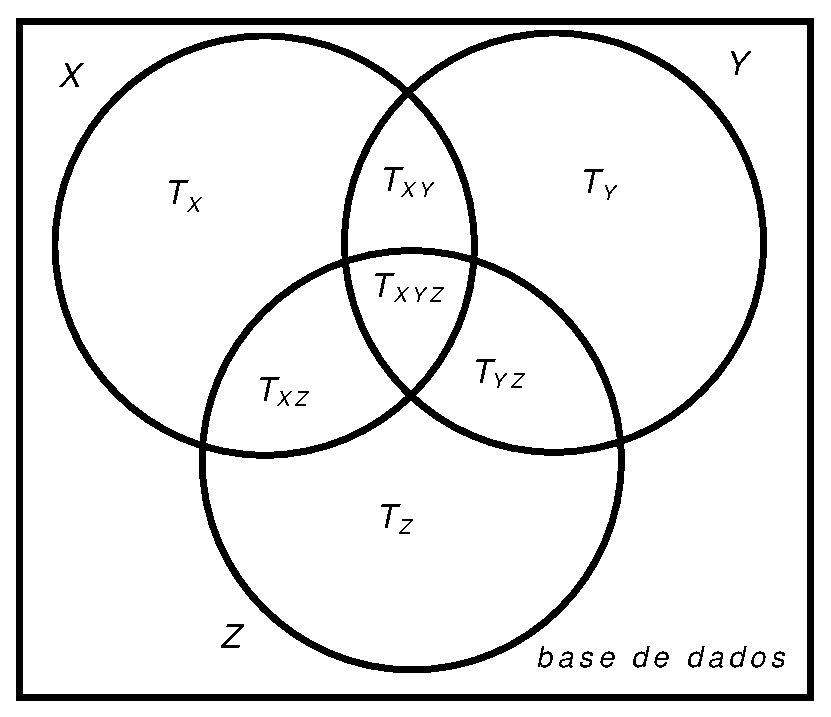
\includegraphics[width=0.5\textwidth]{../thesis/img/coverage}
	\caption{Visualization of Transaction Coverage in the Dataset}
	\label{fig:covex1}
	\end{figure}
\end{frame}

\begin{frame}{Considering Transaction Coverage}
	\begin{itemize}[<+-| alert@+>]
		\item Let $\I$ be a set of items, $\D$ a dataset of transactions in $\I$, $\F$ the set of frequent patterns in $\D$, and $\Fl$ a sub-set of $\F$ ($\Fl \subseteq \F$);
		\item We say that $\Dl \subseteq \D$ is the sub-set of transactions covered by, at least, one of the patterns found in $\Fl$;
		\item For each transaction $t \subseteq \Dl$ is given a weight: \[w_t = \frac{|\Fl| - |\Flt|}{|\Fl| - 1},\] where $\Flt$ is the sub-set of patterns from $\Fl$ that appear in the transaction $t$;
	\end{itemize}
\end{frame}

\begin{frame}{Considering Transaction Coverage}
	\begin{itemize}[<+-| alert@+>]
		\item The orthogonality based in transaction coverage is given by: \[O_t = \frac{\sum_{t \subseteq \Dl} w_t}{|\Dl|}.\]
	\end{itemize}
\end{frame}

\begin{frame}{Considering Class Coverage}
	\begin{block}{Motivation}
		Dois padr�es s�o ortogonais se s�o encontrados em transa��es de classes distintas na base de dados, ou seja, os conjuntos de transa��es cobertas por cada um dos padr�es n�o devem possuir classes em comum.
	\end{block}
\end{frame}

\begin{frame}{Considerando Cobertura de Classes}
	\begin{itemize}[<+-| alert@+>]
		\item Seja $\I$ um conjunto de itens, $\D$ uma base de dados de transa��es em $\I$, $\F$ o conjunto de padr�es freq�entes em $\D$, $\Fl$ um sub-conjunto de $\F$ ($\Fl \subseteq \F$) e $\Dl \subseteq \D$ o sub-conjunto transa��es cobertas por, pelo menos, um dos padr�es de $\Fl$;
		\item Seja $\C$ um conjunto de classes associadas �s transa��es de $\D$ e $\Cl \subseteq \C$ o sub-conjunto de classes associadas �s transa��es de $\Dl$;
		\item Para cada classe $c \subseteq \Cl$ � dado um peso: \[w_c = \frac{|\Fl| - |\Flc|}{|\Fl| - 1},\] onde $\Flc$ � o sub-conjunto de padr�es de $\Fl$ que cobrem uma quantidade de transa��es de classe $c \subseteq \Cl$ maior que $90\%$ da m�dia esperada;		
	\end{itemize}
\end{frame}

%\begin{frame}{Considerando Cobertura de Classes}
%	\begin{itemize}[<+-| alert@+>]
%		\item Para cada classe $c \subseteq \Cl$ � dado um peso: \[w_c = \frac{|\Fl| - |\Flc|}{|\Fl| - 1},\] onde $\Flc$ � o sub-conjunto de padr�es de $\Fl$ que cobrem uma quantidade de transa��es de classe $c \subseteq \Cl$ maior que $90\%$ da m�dia esperada;
%	\end{itemize}
%\end{frame}

\begin{frame}{Considerando Cobertura de Classes}
	\begin{itemize}[<+-| alert@+>]
		\item A ortogonalidade baseada em cobertura de classes � dada por: \[O_c = \frac{\sum_{c \subseteq \Cl} w_c}{|\Cl|}.\]
	\end{itemize}
\end{frame}

\subsection{Classifica��o Associativa e Ortogonalidade}

\begin{frame}{Utiliza��o da ortogonalidade no LAC}
	\begin{itemize}[<+-| alert@+>]
		\item Para cada inst�ncia de teste, o LAC (\textit{Lazy Associative Classifier}) cria uma proje��o da base de treinamento apenas com as transa��es que possuem itens em comum com a inst�ncia;
		\item A partir desta proje��o, a obt�m um conjunto de padr�es freq�entes, de acordo com determinado suporte fornecido pelo usu�rio;
		\item Com estes padr�es, gera as regras de associa��o utilizadas durante a tarefa de classifica��o.
	\end{itemize}
\end{frame}

\begin{frame}{Utiliza��o da ortogonalidade no LAC}
	\begin{itemize}[<+-| alert@+>]
		\item Neste trabalho, a ortogonalidade foi utilizada para se extrair, do conjunto de padr�es freq�entes, um sub-conjunto de padr�es ortogonais;
		\item As regras de associa��o foram geradas a partir do sub-conjunto de padr�es ortogonais obtido.
	\end{itemize}
\end{frame}

\begin{frame}{Heur�stica de Obten��o de Conjuntos Ortogonais}
	\begin{itemize}[<+-| alert@+>]
		\item O problema de se encontrar o sub-conjunto de padr�es com maior m�trica de ortogonalidade, dado o conjunto de padr�es freq�entes, � n�o polinomial;
		\item Foi desenvolvida uma heur�stica gulosa que inicia com um conjunto ortogonal de dois elementos, e, iterativamente, tenta obter um novo conjunto com um elemento a mais, acrescentando padr�es candidatos e realizando modifica��es para que a m�trica de ortogonalidade seja maximizada.
	\end{itemize}
\end{frame}

\begin{frame}[shrink=5]{Heur�stica de Obten��o de Conjuntos Ortogonais}
%\begin{frame}{Heur�stica de Obten��o de Conjuntos Ortogonais}

\begin{algorithm}[H]
\caption{OLAC}
\label{alg:olac}
\begin{algorithmic}[1]

\REQUIRE $\D, \sigma$
	\STATE $\F \leftarrow FindFrequentPatterns (\D, \sigma)$
	\STATE $Sort (\F)$
	\STATE $\Or \leftarrow GetFirstAvailablePattern (\F)$
	\REPEAT
		\STATE $rate \leftarrow GetOrthogonalityRate (\Or)$
%		\STATE $\Or_{try} \leftarrow \Or \cup GetFirstAvailablePattern (\F)$
%		\STATE $rate_{try} = GetOrthogonalityRate (\Or_{try})$
%		\FOR {$P \in \F, P \notin \Or_{try}$}
%			\STATE $S \leftarrow GetMoreSimilar (\Or, P)$
%			\STATE $\Or_{try} \leftarrow \Or_{try} \cup P \ \backslash \ S$
%			\STATE $rate_{tmp} = GetRate (\Or)$
%			\IF {$rate_{tmp} \leq rate_{try}$}
%				\STATE $\Or_{try} \leftarrow \Or_{try} \cup S \  \backslash \  P$
%			\ELSE
%				\STATE $rate_{try} \leftarrow rate_{tmp}$
%			\ENDIF
%		\ENDFOR
		\STATE $\Or_{c} \leftarrow GetNextCandidateSet (\Or, \F)$
		\STATE $rate_{c} = GetOrthogonalityRate (\Or_{c})$
		\IF {$rate_{c} \geq rate$}
			\STATE $\Or \leftarrow \Or_{c}$
		\ENDIF
	\UNTIL {$rate_{c} < rate$}
	\STATE $\R \leftarrow \Or$

\end{algorithmic}
\end{algorithm}

\end{frame}

\begin{frame}[shrink=5]{Heur�stica de Obten��o de Conjuntos Ortogonais}
%\begin{frame}{Heur�stica de Obten��o de Conjuntos Ortogonais}

\begin{algorithm}[H]
\caption{OLAC - GetNextCandidateSet}
\label{alg:olac_getNextCandidateSet}
\begin{algorithmic}[1]

\REQUIRE $\Or, \F$
\STATE $\Or_{c} \leftarrow \Or \cup GetFirstAvailablePattern (\F)$
\STATE $rate_{c} = GetOrthogonalityRate (\Or_{c})$
\FOR {$P \in \F, P \notin \Or_{c}$}
	\STATE $S \leftarrow GetMoreSimilar (\Or_{c}, P)$
	\STATE $\Or_{c} \leftarrow \Or_{c} \cup P \ \backslash \ S$
	\STATE $rate_{try} = GetRate (\Or_{c})$
	\IF {$rate_{try} > rate_{c}$}
		\STATE $rate_{c} \leftarrow rate_{try}$
	\ELSE
		\STATE $\Or_{c} \leftarrow \Or_{c} \cup S \  \backslash \  P$
	\ENDIF
\ENDFOR
\RETURN $\Or_{c}$
%
\end{algorithmic}
\end{algorithm}

\end{frame}

\subsection{Estrat�gia ORIGAMI}

\begin{frame}{Contextualiza��o}
O \textbf{ORIGAMI} � um algoritmo para minera��o de grafos encontrado na literatura, onde os autores introduzem a defini��o de conjuntos $\alpha$-ortogonais e $\beta$-representativos, e apresentam o novo paradigma de minera��o de conjuntos de grafos ortogonais com foco nos padr�es, e n�o nas transa��es.
\end{frame}

\begin{frame}{Defini��o de $\alpha$-ortogonalidade}
	\begin{itemize}[<+-| alert@+>]
		\item Seja $\F$ o conjunto de todos os sub-grafos freq�entes de uma cole��o;
		\item Seja $sim : \F \times \F \rightarrow \left[0, 1\right]$ uma fun��o bin�ria e sim�trica que retorna a \textit{similaridade} entre dois grafos;
		\item Dada uma cole��o de grafos $\G$, e um limite superior para similaridade $\alpha \in \left[0, 1\right]$, dizemos que o sub-conjunto de grafos $\R \subseteq \G$ � \textbf{$\alpha$-ortogonal} em rela��o a $\G$ se, e somente se, para quaisquer $G_a, G_b \in \R, sim(G_a, G_b) \leq \alpha$ e para qualquer $G_a \in \R$ e qualquer $G_b \in \G \backslash \R, sim(G_a, G_b) > \alpha$;
	\end{itemize}
\end{frame}

\begin{frame}{Defini��o de $\alpha$-ortogonalidade}
	\begin{itemize}[<+-| alert@+>]
		\item Dada uma cole��o de grafos $\G$,um conjunto $\alpha$-ortogonal $\R \subseteq \G$ e um limite inferior para similaridade $\beta \in \left[0, 1\right]$, dizemos que $\R$ \textbf{representa} um grafo $G \in \G$ se existe algum $G_a \in \R$ tal que $sim(G_a, G) \geq \beta$. Seja $\Upsilon(\R,\G) = \left\{G \in \G : \exists G_a \in \R, sim(G, G_a) \geq \beta\right\}$, dizemos que $\R$ � um conjunto $\beta$-representativo para $\Upsilon(\R, \G)$;
	\end{itemize}
\end{frame}

\begin{frame}{Defini��o de $\alpha$-ortogonalidade}
	\begin{itemize}[<+-| alert@+>]		
		\item Dada uma cole��o de grafos $\G$ e o seu conjunto $\alpha$-ortogonal e $\beta$-representativo $\R$, chamamos de \textbf{res�duo} de $\R$ o conjunto de padr�es n�o representados em $\G$, dado como $\Delta(\R, \G) = \G \backslash \left\{ \R \cup \Upsilon(\R, \G) \right\}$, o \textit{res�duo} de $\R$ � definido como a cardinalidade do seu conjunto res�duo $|\Delta(\R, \G)|$. Finalmente, definimos a m�dia de similaridade do res�duo de $\R$ como $ars(\R, \G) = \frac{\sum_{G_b \in \Delta(\R, \G)} {max_{G_a \in \R} \left\{sim(G_a, G_b)\right\}}}{|\Delta(\R, \G)|}$.
	\end{itemize}
\end{frame}

\begin{frame}{Defini��o de $\alpha$-ortogonalidade}
	\begin{block}{Objetivo}
		O objetivo � encontrar conjuntos de grafos $\alpha$-ortogonais e $\beta$-representativos em rela��o ao conjunto de sub-grafos maximais $\M$.
	\end{block}
\end{frame}

\begin{frame}{O Algoritmo ORIGAMI}

\begin{algorithm}[H]
\caption{ORIGAMI}
\label{alg:origami}
\begin{algorithmic}[1]

\REQUIRE $\D, \sigma, \alpha, \beta$
\STATE $EM \leftarrow EdgeMap (\D)$
\STATE $\F_1 \leftarrow FindFrequentEdges (\D, \sigma)$
\STATE $\widehat{\M} \leftarrow 0$
\WHILE {$\neg StopCondition ()$}
	\STATE $M \leftarrow RandomMaximalGraph (\D, \F_1, EM, \sigma)$
	\STATE $\widehat{\M} \leftarrow \widehat{\M} \cup M$
\ENDWHILE
\STATE $\R \leftarrow OrthogonalRepresentativeSets (\widehat{\M}, \alpha, \beta)$

\end{algorithmic}
\end{algorithm}

\end{frame}

\begin{frame}{Adapta��o do Algoritmo}
	\begin{itemize}[<+-| alert@+>]
		\item Foi implementada uma adapta��o do ORIGAMI para o problema de Classifica��o Associativa;
		\item Foi implementada uma heur�stica de obten��o de padr�es maximais baseada no trabalho apresentado no artigo;
		\item Foi implementada uma heur�stica de obten��o do conjunto ortogonal baseada no trabalho apresentado no artigo.
	\end{itemize}
\end{frame}

\begin{frame}{Heur�stica de Obten��o de Padr�es Maximais}
	\begin{itemize}[<+-| alert@+>]
		\item O algoritmo inicia a execu��o com o conjunto-resultado vazio;
		\item A cada itera��o, tenta obter o maior padr�o freq�ente poss�vel, selecionando itens aleatoriamente;
			\begin{itemize}[<+-| alert@+>]
				\item Se o algoritmo escolhe um item j� utilizado, ou que produz um padr�o n�o freq�ente, um contador de tentativas � decrementado;
				\item A condi��o de parada para a gera��o do padr�o maximal candidato � que o n�mero de escolhas erradas do item n�o deve ser maior que o tamanho da inst�ncia de teste.
			\end{itemize}
	\end{itemize}
\end{frame}

\begin{frame}{Heur�stica de Obten��o de Padr�es Maximais}
	\begin{itemize}[<+-| alert@+>]
		\item Ao obter um novo padr�o maximal, o algoritmo tenta inseri-lo no conjunto-solu��o;
		\begin{itemize}[<+-| alert@+>]
			\item Se o padr�o escolhido j� existe no conjunto, o algoritmo incrementa um segundo contador de tentativas;
			\item A condi��o de parada para a obten��o de padr�es maximais � que o n�mero de padr�es candidatos n�o maximais ou j� conhecidos n�o deve ser superior ao tamanho da inst�ncia de teste.
		\end{itemize}
	\end{itemize}
\end{frame}

\begin{frame}{Heur�stica de Obten��o do Conjunto Ortogonal}
	\begin{itemize}[<+-| alert@+>]
		\item O algoritmo inicia a execu��o com o valor de res�duo igual a $0$ (zero);
		\item A cada itera��o, tenta obter um novo conjunto ortogonal selecionando, aleatoriamente, padr�es maximais encontrados na primeira fase do algoritmo, e adicionando-os ao conjunto-solu��o;
		\begin{itemize}[<+-| alert@+>]
			\item Se, durante a obten��o dos padr�es, o padr�o selecionado j� ter sido utilizado, ou n�o possuir similaridade menor que $\alpha$ para com todos os outros padr�es do conjunto-solu��o, o algoritmo decrementa um contador de tentativas;
			\item A condi��o de parada local para a gera��o de conjuntos ortogonais � que, durante este processo, o n�mero m�ximo de escolhas erradas de padr�es n�o pode ser maior que a quantidade de padr�es maximais total.
		\end{itemize}
	\end{itemize}
\end{frame}

\begin{frame}{Heur�stica de Obten��o do Conjunto Ortogonal}
	\begin{itemize}[<+-| alert@+>]		
		\item Ao obter um novo conjunto ortogonal, o algoritmo calcula o valor do seu res�duo;
		\item Se este valor � menor que o atual, o res�duo � atualizado, e o conjunto-solu��o passa a ser o conjunto ortogonal rec�m-encontrado;
		\item A condi��o de parada para o algoritmo � que, durante todo o processo, o n�mero m�ximo de conjuntos ortogonais candidatos que n�o melhoram o resultado n�o pode ser maior que a quantidade de padr�es maximais total.
	\end{itemize}
\end{frame}


%\begin{frame}{Heur�stica de Obten��o de Conjuntos Ortogonais}
%	\begin{itemize}[<+-| alert@+>]
%		\item No in�cio do algoritmo, o conjunto-solu��o � inicializado com apenas um elemento, e a m�trica de ortogonalidade do conjunto com o valor $0$ (zero), e ent�o come�a o ciclo de itera��es:
%		\begin{enumerate}[<+-| alert@+>]
%			\item Um novo elemento � inclu�do ao conjunto;
%			\item � realizada uma busca por todo o conjunto de padr�es que n�o fazem parte do conjunto-solu��o. Durante este procedimento, cada padr�o verificado � inclu�do na solu��o, substituindo, neste conjunto, o elemento que mais se assemelha �quele. Se a m�trica de ortogonalidade do conjunto melhorou, o algoritmo mant�m a troca. Se n�o, a troca � desfeita, e o pr�ximo padr�o da seq��ncia � verificado;
%			\item Ao final do processo, o algoritmo compara a m�trica de ortogonalidade obtida com a m�trica do conjunto anterior (que possu�a um elemento a menos). Se a m�trica se manteve, ou melhorou, o algoritmo mant�m o novo conjunto como solu��o, e volta ao in�cio do ciclo. Se n�o, o algoritmo termina o ciclo, e o conjunto anterior � dado como resultado.
%		\end{enumerate}
%	\end{itemize}
%\end{frame}


% M�tricas de Ortogonalidade
% Classifica��o Associativa e Ortogonalidade
% Estrat�gia ORIGAMI

%\section{Padr�es Freq�entes e Ortogonais}
\subsection{Contextualiza��o}

\begin{frame}{Padr�es Freq�entes}
	\begin{itemize}[<+-| alert@+>]
		\item Largamente utilizados em diversas aplica��es, incluindo regras de associa��o, classifica��o, agrupamento, indexa��o, etc.;
		\item Minimizar o conjunto-solu��o ainda � um desafio:
		\begin{itemize}[<+-| alert@+>]
			\item Padr�es freq�entes obedecem � propriedade de anti-monotonia;
			\item Solu��es propostas minimizam o conjunto-solu��o apenas sob a perspectiva do suporte, n�o considerando a sem�ntica dos dados.
		\end{itemize}
		\item Diminuir a redund�ncia no conjunto-solu��o � outro desafio:
		\begin{itemize}[<+-| alert@+>]
			\item Poucos estudos t�m se dedicado a obter sub-conjuntos de alta signific�ncia e baixa redund�ncia ao mesmo tempo.
		\end{itemize}
	\end{itemize}
\end{frame}

\begin{frame}{Padr�es Freq�entes}
	\begin{block}{Padr�es Ortogonais}
		O objetivo da aplica��o de ortogonalidade no problema da minera��o de padr�es freq�entes � desenvolver uma t�cnica capaz de extrair um sub-conjunto de padr�es com tanto alta signific�ncia quanto baixa redund�ncia entre seus elementos.
	\end{block}
\end{frame}

\begin{frame}{M�tricas de Ortogonalidade}
	\begin{itemize}[<+-| alert@+>]
		\item � necess�rio definir m�tricas de ortogonalidade capazes de avaliar um poss�vel conjunto solu��o;
		\item O complemento do coeficiente de \textbf{Jaccard} aplicado � cobertura da base de dados pode ser considerado como uma m�trica de ortogonalidade entre dois padr�es: \[D(p_1,p_2) = 1 - \frac{|TS(p_1) \cap TS(p_2)|}{|TS(p_1) \cup TS(p_2)|},\] onde $TS(p)$ � o conjunto de transa��es cobertas por $p$.
		\item Estamos interessados em definir m�tricas aplic�veis a conjuntos de qualquer tamanho.
	\end{itemize}
\end{frame}

\subsection{M�tricas de Ortogonalidade}

\begin{frame}{Considerando Estrutura dos Padr�es}
	\begin{block}{Motiva��o}
		Dois padr�es s�o ortogonais se eles n�o possuem itens em comum, ou seja, pode-se dizer que os padr�es $ABC$ e $DEF$ s�o ortogonais, mas $ABC$ e $CDE$ n�o o s�o, j� que o item $C$ est� presente nos dois padr�es. O mesmo pode ser aplicado a conjuntos maiores, por exemplo, os padr�es $AB$, $CD$ e $EF$ s�o ortogonais, mas os padr�es $AB$, $BC$ e $CD$ n�o o s�o.
	\end{block}
\end{frame}
\begin{frame}{Considerando Estrutura dos Padr�es}
	\begin{itemize}[<+-| alert@+>]
		\item Seja $\I$ um conjunto de itens, $\D$ uma base de dados de transa��es em $\I$, $\F$ o conjunto de padr�es freq�entes em $\D$, e $\Fl$ um sub-conjunto de $\F$ ($\Fl \subseteq \F$);
		\item Chamamos de $\Il \subseteq \I$ o sub-conjunto itens que aparecem em, pelo menos, um dos padr�es de $\Fl$;
		\item Para cada item $i \subseteq \Il$ � dado um peso: \[w_i = \frac{|\Fl|-|\Fli|}{|\Fl|-1},\] onde $\Fli \subseteq \Fl$ � o sub-conjunto de padr�es de $\Fl$ que cont�m o item $i$;
	\end{itemize}
\end{frame}

\begin{frame}{Considerando Estrutura dos Padr�es}
	\begin{itemize}[<+-| alert@+>]
		\item A ortogonalidade baseada na estrutura dos padr�es do conjunto � dada por: \[O_e = \frac{\sum_{i \subseteq \Il} w_i}{|\Il|}.\]
	\end{itemize}
\end{frame}

\begin{frame}{Considerando Cobertura de Transa��es}
	\begin{block}{Motiva��o}
		Dois padr�es s�o ortogonais se eles cobrem �reas diferentes da base de dados, ou seja, se os conjuntos de transa��es cobertas por cada padr�o n�o possuem elementos em comum.
	\end{block}
\end{frame}

\begin{frame}{Considerando Cobertura de Transa��es}
	\begin{figure}
	\centering
	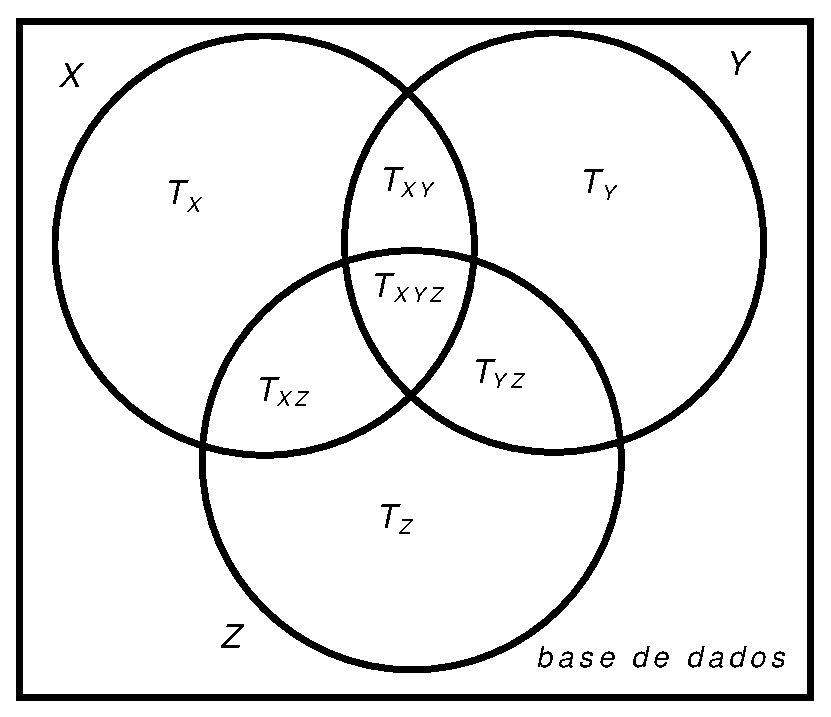
\includegraphics[width=0.5\textwidth]{../thesis/img/coverage}
	\caption{Visualiza��o de Cobertura de Transa��es na Base de Dados}
	\label{fig:covex1}
	\end{figure}
\end{frame}

\begin{frame}{Considerando Cobertura de Transa��es}
	\begin{itemize}[<+-| alert@+>]
		\item Seja $\I$ um conjunto de itens, $\D$ uma base de dados de transa��es em $\I$, $\F$ o conjunto de padr�es freq�entes em $\D$, e $\Fl$ um sub-conjunto de $\F$ ($\Fl \subseteq \F$);
		\item Chamamos de $\Dl \subseteq \D$ o sub-conjunto transa��es cobertas por, pelo menos, um dos padr�es de $\Fl$;
		\item Para cada transa��o $t \subseteq \Dl$ � dado um peso: \[w_t = \frac{|\Fl| - |\Flt|}{|\Fl| - 1},\] onde $\Flt$ � o sub-conjunto de padr�es de $\Fl$ que cobrem a transa��o $t$;
	\end{itemize}
\end{frame}

\begin{frame}{Considerando Cobertura de Transa��es}
	\begin{itemize}[<+-| alert@+>]
		\item A ortogonalidade baseada em cobertura de transa��es do conjunto � dada por: \[O_t = \frac{\sum_{t \subseteq \Dl} w_t}{|\Dl|}.\]
	\end{itemize}
\end{frame}

\begin{frame}{Considerando Cobertura de Classes}
	\begin{block}{Motiva��o}
		Dois padr�es s�o ortogonais se s�o encontrados em transa��es de classes distintas na base de dados, ou seja, os conjuntos de transa��es cobertas por cada um dos padr�es n�o devem possuir classes em comum.
	\end{block}
\end{frame}

\begin{frame}{Considerando Cobertura de Classes}
	\begin{itemize}[<+-| alert@+>]
		\item Seja $\I$ um conjunto de itens, $\D$ uma base de dados de transa��es em $\I$, $\F$ o conjunto de padr�es freq�entes em $\D$, $\Fl$ um sub-conjunto de $\F$ ($\Fl \subseteq \F$) e $\Dl \subseteq \D$ o sub-conjunto transa��es cobertas por, pelo menos, um dos padr�es de $\Fl$;
		\item Seja $\C$ um conjunto de classes associadas �s transa��es de $\D$ e $\Cl \subseteq \C$ o sub-conjunto de classes associadas �s transa��es de $\Dl$;
		\item Para cada classe $c \subseteq \Cl$ � dado um peso: \[w_c = \frac{|\Fl| - |\Flc|}{|\Fl| - 1},\] onde $\Flc$ � o sub-conjunto de padr�es de $\Fl$ que cobrem uma quantidade de transa��es de classe $c \subseteq \Cl$ maior que $90\%$ da m�dia esperada;		
	\end{itemize}
\end{frame}

%\begin{frame}{Considerando Cobertura de Classes}
%	\begin{itemize}[<+-| alert@+>]
%		\item Para cada classe $c \subseteq \Cl$ � dado um peso: \[w_c = \frac{|\Fl| - |\Flc|}{|\Fl| - 1},\] onde $\Flc$ � o sub-conjunto de padr�es de $\Fl$ que cobrem uma quantidade de transa��es de classe $c \subseteq \Cl$ maior que $90\%$ da m�dia esperada;
%	\end{itemize}
%\end{frame}

\begin{frame}{Considerando Cobertura de Classes}
	\begin{itemize}[<+-| alert@+>]
		\item A ortogonalidade baseada em cobertura de classes � dada por: \[O_c = \frac{\sum_{c \subseteq \Cl} w_c}{|\Cl|}.\]
	\end{itemize}
\end{frame}

\subsection{Classifica��o Associativa e Ortogonalidade}

\begin{frame}{Utiliza��o da ortogonalidade no LAC}
	\begin{itemize}[<+-| alert@+>]
		\item Para cada inst�ncia de teste, o LAC (\textit{Lazy Associative Classifier}) cria uma proje��o da base de treinamento apenas com as transa��es que possuem itens em comum com a inst�ncia;
		\item A partir desta proje��o, a obt�m um conjunto de padr�es freq�entes, de acordo com determinado suporte fornecido pelo usu�rio;
		\item Com estes padr�es, gera as regras de associa��o utilizadas durante a tarefa de classifica��o.
	\end{itemize}
\end{frame}

\begin{frame}{Utiliza��o da ortogonalidade no LAC}
	\begin{itemize}[<+-| alert@+>]
		\item Neste trabalho, a ortogonalidade foi utilizada para se extrair, do conjunto de padr�es freq�entes, um sub-conjunto de padr�es ortogonais;
		\item As regras de associa��o foram geradas a partir do sub-conjunto de padr�es ortogonais obtido.
	\end{itemize}
\end{frame}

\begin{frame}{Heur�stica de Obten��o de Conjuntos Ortogonais}
	\begin{itemize}[<+-| alert@+>]
		\item O problema de se encontrar o sub-conjunto de padr�es com maior m�trica de ortogonalidade, dado o conjunto de padr�es freq�entes, � n�o polinomial;
		\item Foi desenvolvida uma heur�stica gulosa que inicia com um conjunto ortogonal de dois elementos, e, iterativamente, tenta obter um novo conjunto com um elemento a mais, acrescentando padr�es candidatos e realizando modifica��es para que a m�trica de ortogonalidade seja maximizada.
	\end{itemize}
\end{frame}

\begin{frame}[shrink=5]{Heur�stica de Obten��o de Conjuntos Ortogonais}
%\begin{frame}{Heur�stica de Obten��o de Conjuntos Ortogonais}

\begin{algorithm}[H]
\caption{OLAC}
\label{alg:olac}
\begin{algorithmic}[1]

\REQUIRE $\D, \sigma$
	\STATE $\F \leftarrow FindFrequentPatterns (\D, \sigma)$
	\STATE $Sort (\F)$
	\STATE $\Or \leftarrow GetFirstAvailablePattern (\F)$
	\REPEAT
		\STATE $rate \leftarrow GetOrthogonalityRate (\Or)$
%		\STATE $\Or_{try} \leftarrow \Or \cup GetFirstAvailablePattern (\F)$
%		\STATE $rate_{try} = GetOrthogonalityRate (\Or_{try})$
%		\FOR {$P \in \F, P \notin \Or_{try}$}
%			\STATE $S \leftarrow GetMoreSimilar (\Or, P)$
%			\STATE $\Or_{try} \leftarrow \Or_{try} \cup P \ \backslash \ S$
%			\STATE $rate_{tmp} = GetRate (\Or)$
%			\IF {$rate_{tmp} \leq rate_{try}$}
%				\STATE $\Or_{try} \leftarrow \Or_{try} \cup S \  \backslash \  P$
%			\ELSE
%				\STATE $rate_{try} \leftarrow rate_{tmp}$
%			\ENDIF
%		\ENDFOR
		\STATE $\Or_{c} \leftarrow GetNextCandidateSet (\Or, \F)$
		\STATE $rate_{c} = GetOrthogonalityRate (\Or_{c})$
		\IF {$rate_{c} \geq rate$}
			\STATE $\Or \leftarrow \Or_{c}$
		\ENDIF
	\UNTIL {$rate_{c} < rate$}
	\STATE $\R \leftarrow \Or$

\end{algorithmic}
\end{algorithm}

\end{frame}

\begin{frame}[shrink=5]{Heur�stica de Obten��o de Conjuntos Ortogonais}
%\begin{frame}{Heur�stica de Obten��o de Conjuntos Ortogonais}

\begin{algorithm}[H]
\caption{OLAC - GetNextCandidateSet}
\label{alg:olac_getNextCandidateSet}
\begin{algorithmic}[1]

\REQUIRE $\Or, \F$
\STATE $\Or_{c} \leftarrow \Or \cup GetFirstAvailablePattern (\F)$
\STATE $rate_{c} = GetOrthogonalityRate (\Or_{c})$
\FOR {$P \in \F, P \notin \Or_{c}$}
	\STATE $S \leftarrow GetMoreSimilar (\Or_{c}, P)$
	\STATE $\Or_{c} \leftarrow \Or_{c} \cup P \ \backslash \ S$
	\STATE $rate_{try} = GetRate (\Or_{c})$
	\IF {$rate_{try} > rate_{c}$}
		\STATE $rate_{c} \leftarrow rate_{try}$
	\ELSE
		\STATE $\Or_{c} \leftarrow \Or_{c} \cup S \  \backslash \  P$
	\ENDIF
\ENDFOR
\RETURN $\Or_{c}$
%
\end{algorithmic}
\end{algorithm}

\end{frame}

\setbeamercovered{invisible}

\begin{frame}{Exemplo de Execu��o da Heur�stica}

	\begin{overprint}
		\onslide<2-5>
			Padr�es Freq�entes: \{\alert<5>{ABC},BC,A,B\}
		\onslide<6-8>
			Padr�es Freq�entes: \{\st{ABC},\alert<8>{BC},A,B\}
		\onslide<9-14>
			Padr�es Freq�entes: \{\st{ABC},\st{BC},\alert<11-14>{A},B\}
		\onslide<15-22>
			Padr�es Freq�entes: \{\alert<22>{ABC},\st{BC},\st{A},\alert<16-19>{B}\}
		\onslide<23-28>
			Padr�es Freq�entes: \{\st{ABC},\st{BC},\st{A},\alert<25-28>{B}\}
		\onslide<29>
			Padr�es Freq�entes: \{\st{ABC},BC,\st{A},\st{B}\}
		\onslide<30>
			Padr�es Freq�entes: \{ABC,BC,A,B\}
	\end{overprint}
	
	\begin{overprint}
		\onslide<3-5>
			Padr�es Ortogonais: \{\}
		\onslide<6-8>
			Padr�es Ortogonais: \{ABC\}
		\onslide<9-14>
			Padr�es Ortogonais: \{\alert<12-14>{ABC},BC\}
		\onslide<15-22>
			Padr�es Ortogonais: \{A,\alert<17-19>{BC}\}
		\onslide<23-28>
			Padr�es Ortogonais: \{A,\alert<26-28>{BC},ABC\}
		\onslide<29>
			Padr�es Ortogonais: \{A,B,ABC\}
	\end{overprint}
	\begin{overprint}
		\onslide<4-9>
			Ortogonalidade: $-$
		\onslide<10-14>
			Ortogonalidade: \alert<14>{$0.33$}
		\onslide<15-23>
			Ortogonalidade: \alert<19-20>{$1$}
		\onslide<24-28>
			Ortogonalidade: \alert<28-29>{$0.5$}
		\onslide<29>
			Ortogonalidade: \alert<29>{$0.67$}
	\end{overprint}
	
	\hspace{1cm}
	
	\begin{overprint}
		\onslide<13-14>
			Padr�es Ortogonais (c): \{A,BC\}
		\onslide<18-19>
			Padr�es Ortogonais (c): \{A,B\}
		\onslide<27-28>
			Padr�es Ortogonais (c): \{A,B,ABC\}
	\end{overprint}
	\begin{overprint}
		\onslide<14>
			Ortogonalidade (c): \alert<14>{$1$}
		\onslide<19>
			Ortogonalidade (c): \alert<19>{$1$}
		\onslide<28>
			Ortogonalidade (c): \alert<28>{$0.67$}
	\end{overprint}
	
	\hspace{1cm}
	
	\begin{overprint}
		\onslide<7-20>
			Padr�es Ortogonais (r): \{ABC\}
		\onslide<21-30>
			Padr�es Ortogonais (r): \alert<30>{\{A,BC\}}
	\end{overprint}
	\begin{overprint}
		\onslide<7-20>
			Ortogonalidade (r): \alert<20>{$0$}
		\onslide<21-30>
			Ortogonalidade (r): \alert<29-30>{$1$}
	\end{overprint}

\end{frame}

\setbeamercovered{transparent}

\subsection{Estrat�gia ORIGAMI}

\begin{frame}{Contextualiza��o}
O \textbf{ORIGAMI} � um algoritmo para minera��o de grafos encontrado na literatura, onde os autores introduzem a defini��o de conjuntos $\alpha$-ortogonais e $\beta$-representativos, e apresentam o novo paradigma de minera��o de conjuntos de grafos ortogonais com foco nos padr�es, e n�o nas transa��es.
\end{frame}

\begin{frame}{Defini��o de $\alpha$-ortogonalidade}
	\begin{itemize}[<+-| alert@+>]
		\item Seja $\F$ o conjunto de todos os sub-grafos freq�entes de uma cole��o;
		\item Seja $sim : \F \times \F \rightarrow \left[0, 1\right]$ uma fun��o bin�ria e sim�trica que retorna a \textit{similaridade} entre dois grafos;
		\item Dada uma cole��o de grafos $\G$, e um limite superior para similaridade $\alpha \in \left[0, 1\right]$, dizemos que o sub-conjunto de grafos $\R \subseteq \G$ � \textbf{$\alpha$-ortogonal} em rela��o a $\G$ se, e somente se, para quaisquer $G_a, G_b \in \R, sim(G_a, G_b) \leq \alpha$ e para qualquer $G_a \in \R$ e qualquer $G_b \in \G \backslash \R, sim(G_a, G_b) > \alpha$;
	\end{itemize}
\end{frame}

\begin{frame}{Defini��o de $\alpha$-ortogonalidade}
	\begin{itemize}[<+-| alert@+>]
		\item Dada uma cole��o de grafos $\G$,um conjunto $\alpha$-ortogonal $\R \subseteq \G$ e um limite inferior para similaridade $\beta \in \left[0, 1\right]$, dizemos que $\R$ \textbf{representa} um grafo $G \in \G$ se existe algum $G_a \in \R$ tal que $sim(G_a, G) \geq \beta$. Seja $\Upsilon(\R,\G) = \left\{G \in \G : \exists G_a \in \R, sim(G, G_a) \geq \beta\right\}$, dizemos que $\R$ � um conjunto $\beta$-representativo para $\Upsilon(\R, \G)$;
	\end{itemize}
\end{frame}

\begin{frame}{Defini��o de $\alpha$-ortogonalidade}
	\begin{itemize}[<+-| alert@+>]		
		\item Dada uma cole��o de grafos $\G$ e o seu conjunto $\alpha$-ortogonal e $\beta$-representativo $\R$, chamamos de \textbf{res�duo} de $\R$ o conjunto de padr�es n�o representados em $\G$, dado como $\Delta(\R, \G) = \G \backslash \left\{ \R \cup \Upsilon(\R, \G) \right\}$, o \textit{res�duo} de $\R$ � definido como a cardinalidade do seu conjunto res�duo $|\Delta(\R, \G)|$. Finalmente, definimos a m�dia de similaridade do res�duo de $\R$ como $ars(\R, \G) = \frac{\sum_{G_b \in \Delta(\R, \G)} {max_{G_a \in \R} \left\{sim(G_a, G_b)\right\}}}{|\Delta(\R, \G)|}$.
	\end{itemize}
\end{frame}

\begin{frame}{Defini��o de $\alpha$-ortogonalidade}
	\begin{block}{Objetivo}
		O objetivo � encontrar conjuntos de grafos $\alpha$-ortogonais e $\beta$-representativos em rela��o ao conjunto de sub-grafos maximais $\M$.
	\end{block}
\end{frame}

\begin{frame}{O Algoritmo ORIGAMI}

\begin{algorithm}[H]
\caption{ORIGAMI}
\label{alg:origami}
\begin{algorithmic}[1]

\REQUIRE $\D, \sigma, \alpha, \beta$
\STATE $EM \leftarrow EdgeMap (\D)$
\STATE $\F_1 \leftarrow FindFrequentEdges (\D, \sigma)$
\STATE $\widehat{\M} \leftarrow 0$
\WHILE {$\neg StopCondition ()$}
	\STATE $M \leftarrow RandomMaximalGraph (\D, \F_1, EM, \sigma)$
	\STATE $\widehat{\M} \leftarrow \widehat{\M} \cup M$
\ENDWHILE
\STATE $\R \leftarrow OrthogonalRepresentativeSets (\widehat{\M}, \alpha, \beta)$

\end{algorithmic}
\end{algorithm}

\end{frame}

\begin{frame}{Adapta��o do Algoritmo}
	\begin{itemize}[<+-| alert@+>]
		\item Foi implementada uma adapta��o do ORIGAMI para o problema de Classifica��o Associativa;
		\item Foi implementada uma heur�stica de obten��o de padr�es maximais baseada no trabalho apresentado no artigo;
		\item Foi implementada uma heur�stica de obten��o do conjunto ortogonal baseada no trabalho apresentado no artigo.
	\end{itemize}
\end{frame}

\begin{frame}{Heur�stica de Obten��o de Padr�es Maximais}
	\begin{itemize}[<+-| alert@+>]
		\item O algoritmo inicia a execu��o com o conjunto-resultado vazio;
		\item A cada itera��o, tenta obter o maior padr�o freq�ente poss�vel, selecionando itens aleatoriamente;
			\begin{itemize}[<+-| alert@+>]
				\item Se o algoritmo escolhe um item j� utilizado, ou que produz um padr�o n�o freq�ente, um contador de tentativas � decrementado;
				\item A condi��o de parada para a gera��o do padr�o maximal candidato � que o n�mero de escolhas erradas do item n�o deve ser maior que o tamanho da inst�ncia de teste.
			\end{itemize}
	\end{itemize}
\end{frame}

\begin{frame}{Heur�stica de Obten��o de Padr�es Maximais}
	\begin{itemize}[<+-| alert@+>]
		\item Ao obter um novo padr�o maximal, o algoritmo tenta inseri-lo no conjunto-solu��o;
		\begin{itemize}[<+-| alert@+>]
			\item Se o padr�o escolhido j� existe no conjunto, o algoritmo incrementa um segundo contador de tentativas;
			\item A condi��o de parada para a obten��o de padr�es maximais � que o n�mero de padr�es candidatos n�o maximais ou j� conhecidos n�o deve ser superior ao tamanho da inst�ncia de teste.
		\end{itemize}
	\end{itemize}
\end{frame}

\begin{frame}{Heur�stica de Obten��o do Conjunto Ortogonal}
	\begin{itemize}[<+-| alert@+>]
		\item O algoritmo inicia a execu��o com o valor de res�duo igual a $0$ (zero);
		\item A cada itera��o, tenta obter um novo conjunto ortogonal selecionando, aleatoriamente, padr�es maximais encontrados na primeira fase do algoritmo, e adicionando-os ao conjunto-solu��o;
		\begin{itemize}[<+-| alert@+>]
			\item Se, durante a obten��o dos padr�es, o padr�o selecionado j� ter sido utilizado, ou n�o possuir similaridade menor que $\alpha$ para com todos os outros padr�es do conjunto-solu��o, o algoritmo decrementa um contador de tentativas;
			\item A condi��o de parada local para a gera��o de conjuntos ortogonais � que, durante este processo, o n�mero m�ximo de escolhas erradas de padr�es n�o pode ser maior que a quantidade de padr�es maximais total.
		\end{itemize}
	\end{itemize}
\end{frame}

\begin{frame}{Heur�stica de Obten��o do Conjunto Ortogonal}
	\begin{itemize}[<+-| alert@+>]		
		\item Ao obter um novo conjunto ortogonal, o algoritmo calcula o valor do seu res�duo;
		\item Se este valor � menor que o atual, o res�duo � atualizado, e o conjunto-solu��o passa a ser o conjunto ortogonal rec�m-encontrado;
		\item A condi��o de parada para o algoritmo � que, durante todo o processo, o n�mero m�ximo de conjuntos ortogonais candidatos que n�o melhoram o resultado n�o pode ser maior que a quantidade de padr�es maximais total.
	\end{itemize}
\end{frame}


%\begin{frame}{Heur�stica de Obten��o de Conjuntos Ortogonais}
%	\begin{itemize}[<+-| alert@+>]
%		\item No in�cio do algoritmo, o conjunto-solu��o � inicializado com apenas um elemento, e a m�trica de ortogonalidade do conjunto com o valor $0$ (zero), e ent�o come�a o ciclo de itera��es:
%		\begin{enumerate}[<+-| alert@+>]
%			\item Um novo elemento � inclu�do ao conjunto;
%			\item � realizada uma busca por todo o conjunto de padr�es que n�o fazem parte do conjunto-solu��o. Durante este procedimento, cada padr�o verificado � inclu�do na solu��o, substituindo, neste conjunto, o elemento que mais se assemelha �quele. Se a m�trica de ortogonalidade do conjunto melhorou, o algoritmo mant�m a troca. Se n�o, a troca � desfeita, e o pr�ximo padr�o da seq��ncia � verificado;
%			\item Ao final do processo, o algoritmo compara a m�trica de ortogonalidade obtida com a m�trica do conjunto anterior (que possu�a um elemento a menos). Se a m�trica se manteve, ou melhorou, o algoritmo mant�m o novo conjunto como solu��o, e volta ao in�cio do ciclo. Se n�o, o algoritmo termina o ciclo, e o conjunto anterior � dado como resultado.
%		\end{enumerate}
%	\end{itemize}
%\end{frame}


% M�tricas de Ortogonalidade
% Classifica��o Associativa e Ortogonalidade
% Estrat�gia ORIGAMI

\section{Evaluation}
\subsection{Experiments}

\begin{frame}{The Applicative \textbf{olac}}
	\begin{itemize}[<+-| alert@+>]
		\item In the applicative \textbf{olac} we have the implementation of three different approaches of an association rules based classifier:
		\begin{itemize}[<+-| alert@+>]
			\item The LAC (\textit{Lazy Associative Classifier}) approach, that is the \textit{lazy} strategy in his original version(and non-orthogonal);
			\item The OLAC (\textit{Orthogonal Lazy Associative Classifier}) approach, that is a variant of the \textit{lazy} strategy considering orthogonality;
			\item The ORIGAMI, that is the adaptation presented for the ORIGAMI strategy.
		\end{itemize}
	\end{itemize}
\end{frame}

%\begin{frame}[fragile,shrink=30]{Op��es de Execu��o}
%
%\begin{verbatim}
%Usage: ./olac [options]
%Options:
%  -i, --training-file       Set the training file
%  -t, --testing-file        Set the testing file
%  -s, --support             Set the support
%  -c, --confidence          Set the confidence
%  -r, --run-mode            Set the run mode [c,o] [CLASSICAL, ORTHOGONAL]
%  -p, --pattern-set         Set the pattern set type [f,m,r] [FREQUENT, MAXIMAL,
%                              RANDOM MAXIMAL]
%  -n, --min-num-rules       Set the minimum number of rules generated
%  -l, --max-num-rank-rules  Set the maximum number of rules considered (rank size)
%  -m, --min-rule-len        Set the minimum length of the rules
%  -x, --max-rule-len        Set the maximum length of the rules
%  -o, --orth-mode           Set the orthogonality mode [h,p,o] [HEURISTICAL,
%                              POLYNOMIAL, ORIGAMI]
%\end{verbatim}
%
%\end{frame}

%\begin{frame}[fragile,shrink=30]{Op��es de Execu��o}
%
%\begin{verbatim}
%  -e, --orth-metric         Set the orthogonality metric [s,c,l,a] [STRUCTURE,
%                              TRANSACTION COVERAGE, CLASS COVERAGE, ALL]
%  -w, --orth-method         Set the way metrics are used [s,p,a] [SET, PAIR AVERAGE,
%                              ALL]
%  -g, --orth-pat-ordering   Set the way patterns are ordered for heuristic
%                              [s,r,i,z,n] [SORTED, REVERSE SORTED, SORTED BY SIZE,
%                              REVERSE SORTED BY SIZE, NONE]
%  -u, --rule-measure        Set the rule measure used [s,c,j,k,o,n,e,p,l,i,v]
%                              [SUPPORT, CONFIDENCE, JACCARD, KULC, COSINE,
%                              CONVICTION, SENSITIVITY, SPECIFICITY, LAPLACE,
%                              LIFT, LEVERAGE]
%  -a, --origami-alpha       Set the alpha parameter used by ORIGAMI
%  -b, --origami-beta        Set the beta parameter used by ORIGAMI
%  -d, --debug               Set the level of debug [-1,0,1,2,3,4] [SILENT, NO DEBUG,
%                              LOW LEVEL, MEDIUM LEVL, HIGH LEVEL, MAX LEVEL]
%  -v, --verbose             Use verbose mode
%  -h, --help                Display this information
%\end{verbatim}
%
%\end{frame}

%\subsection{Experimentos}

\begin{frame}{Methodology}
	\begin{itemize}[<+-| alert@+>]
		\item We used 26 datasets from \textbf{UCI} (\textit{UC Irvine Machine Learning Repository});
		\item We used 10-fold cross-validation and the final results of each experiment represent the average of the ten runs.
			\end{itemize}
\end{frame}

%\begin{frame}{Metodologia}
%	\begin{itemize}[<+-| alert@+>]
%		\item Como resultados foram considerados a m�dia das dez execu��es diferentes para cada base de dados;
%		\item Os par�metros utilizados nos testes se encontram na tabela \ref{tab:table_test_parms_presentation};
%		\item Todas as combina��es poss�veis destes par�metros foram realizadas, com exce��o da combina��o tamanho m�ximo de regra  $1$ e m�trica de ortogonalidade $s$ para o OLAC.
%	\end{itemize}
%\end{frame}

\begin{frame}[shrink]{Methodology}
	\begin{centering}
	\begin{table}[htbp]
	\centering
		\resizebox{0.95\textwidth}{!} {
		\begin{tabular}{|l|c|}
		\hline
		\textbf{Parameters}	& \textbf{Values}	\\
		\hline
		support			& $\left\{ 0.0001, 0.001, 0.01, 0.1, 0.2, 0.3, 0.4, 0.5, 0.6, 0.7, 0.8, 0.9, 0.95, 0.99, 1 \right\}$	\\
		\hline
		confidence		& $\left\{ 0.0001, 0.001, 0.01, 0.1, 0.2, 0.3, 0.4, 0.5, 0.6, 0.7, 0.8, 0.9, 0.95, 0.99, 1 \right\}$				\\
		\hline
		min-num-rules		& $\left\{ 1 \right\}$				\\
		\hline
		max-num-rank-rules	& $\left\{ 1,10,100,1000,10000,100000,1000000 \right\}$		\\
		\hline
		min-rule-len		& $\left\{ 1 \right\}$				\\
		\hline
		max-rule-len		& $\left\{ 1,2,3 \right\}$		\\
		\hline
		rule-measure		& $\left\{ s,c,j,k,o,n,e,p,l,i,v \right\}$	\\
		\hline
		orth-metric		& $\left\{ e,c,l,a \right\}$			\\
		\hline
		orth-method		& $\left\{ s,p \right\}$				\\
		\hline
		orth-pat-ordering	& $\left\{ s,r,i,z,n \right\}$			\\
		\hline
		origami-alpha		& $\left\{ 0.1,0.2,0.3,0.4,0.5,0.6,0.7,0.8,0.9 \right\}$		\\
		\hline
		origami-beta		& $\left\{ 0.1,0.2,0.3,0.4,0.5,0.6,0.7,0.8,0.9 \right\}$		\\
		\hline
		\end{tabular}
		}
	\caption{Parameters Used for All Approaches}
	\label{tab:table_test_parms}
\end{table}

	\end{centering}
\end{frame}

\begin{frame}[shrink]{Better Results for Each Dataset}
	\begin{centering}
	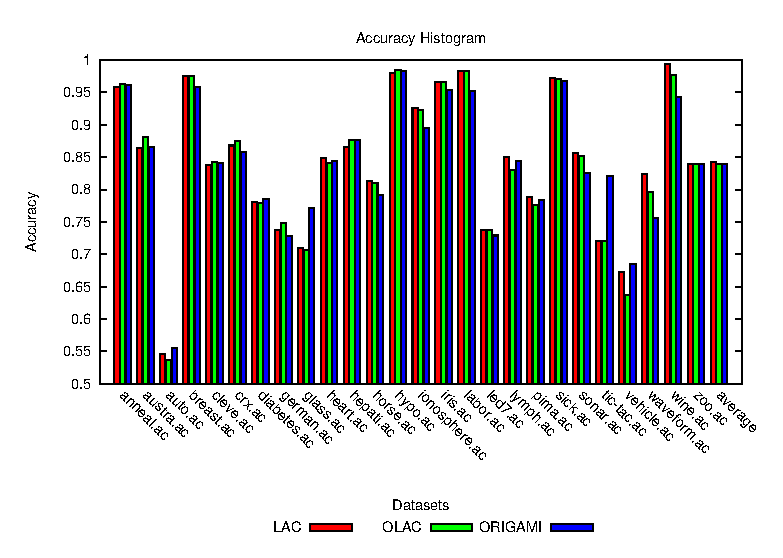
\includegraphics[width=\textwidth]{../thesis/graphs/histogram_best_run_for_each_db_acc_en}
	\end{centering}
\end{frame}

\begin{frame}[shrink]{Better Results for Each Dataset}
	\begin{centering}
	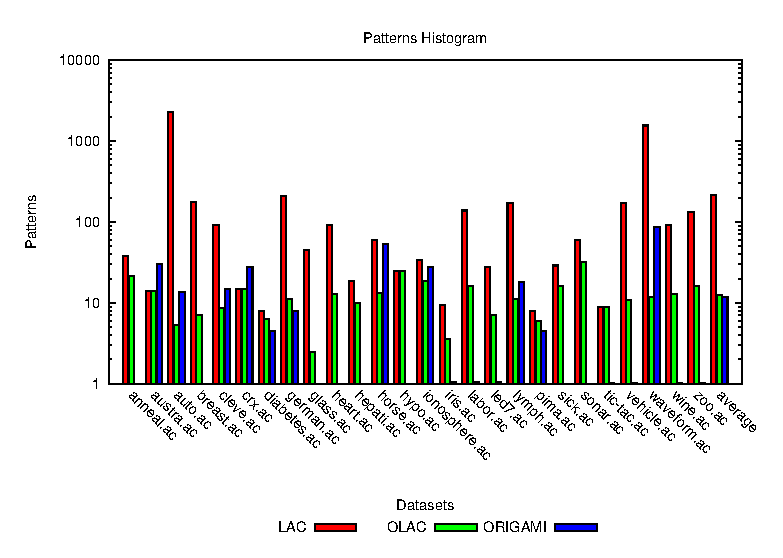
\includegraphics[width=\textwidth]{../thesis/graphs/histogram_best_run_for_each_db_pat_en}
	\end{centering}
\end{frame}

\begin{frame}[shrink]{Better Results for Each Dataset}
	\begin{centering}
	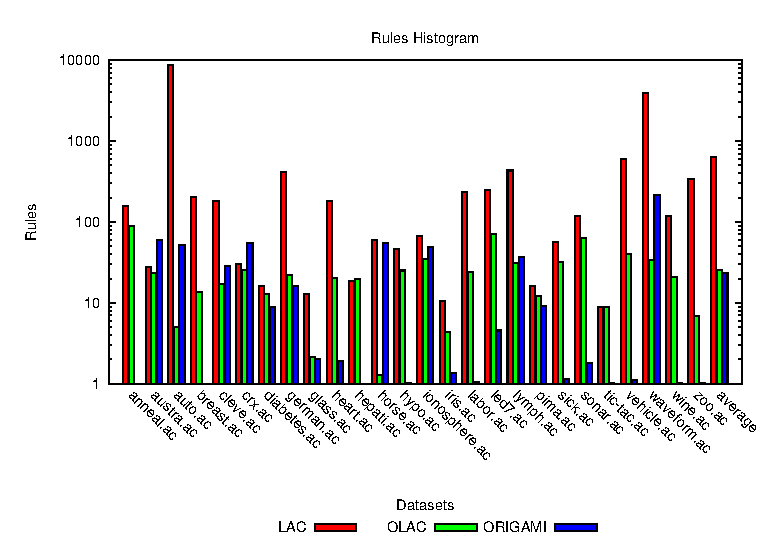
\includegraphics[width=\textwidth]{../thesis/graphs/histogram_best_run_for_each_db_rul_en}
	\end{centering}
\end{frame}

\begin{frame}[shrink]{Better Results in Average for All Datasets}
	\begin{centering}
	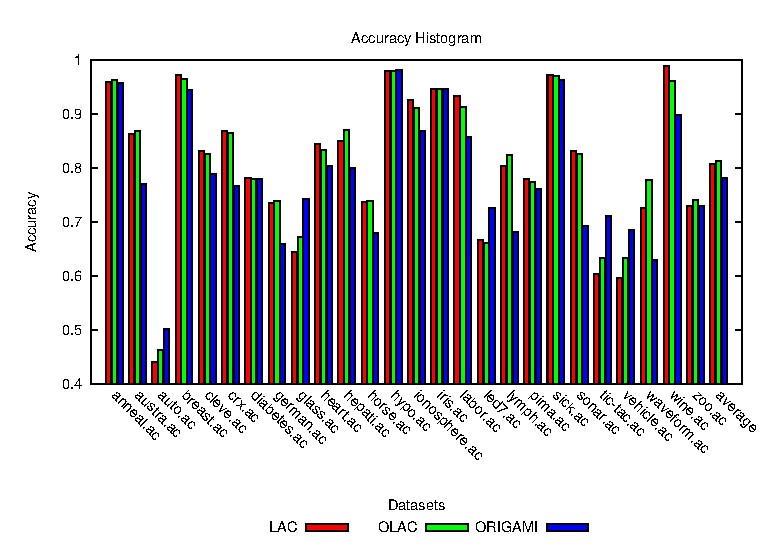
\includegraphics[width=\textwidth]{../thesis/graphs/histogram_best_run_for_avg_db_acc_en}
	\end{centering}
\end{frame}

\begin{frame}[shrink]{Better Results in Average for All Datasets}
	\begin{centering}
	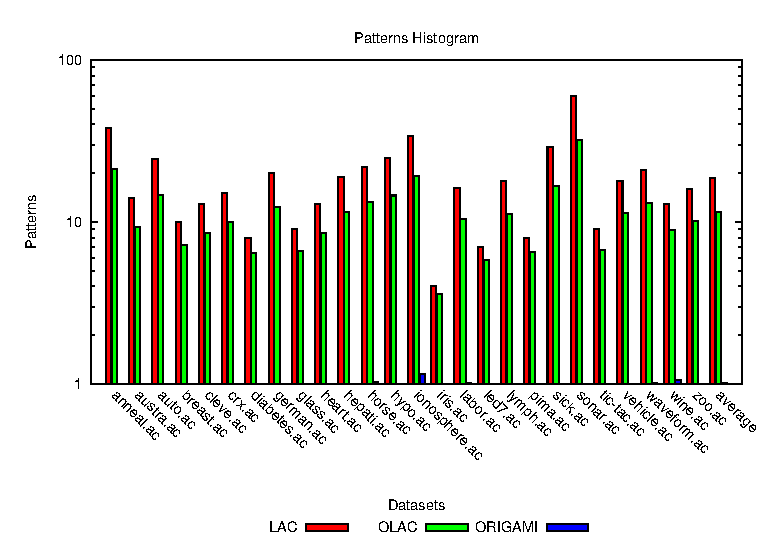
\includegraphics[width=\textwidth]{../thesis/graphs/histogram_best_run_for_avg_db_pat_en}
	\end{centering}
\end{frame}

\begin{frame}[shrink]{Better Results in Average for All Datasets}
	\begin{centering}
	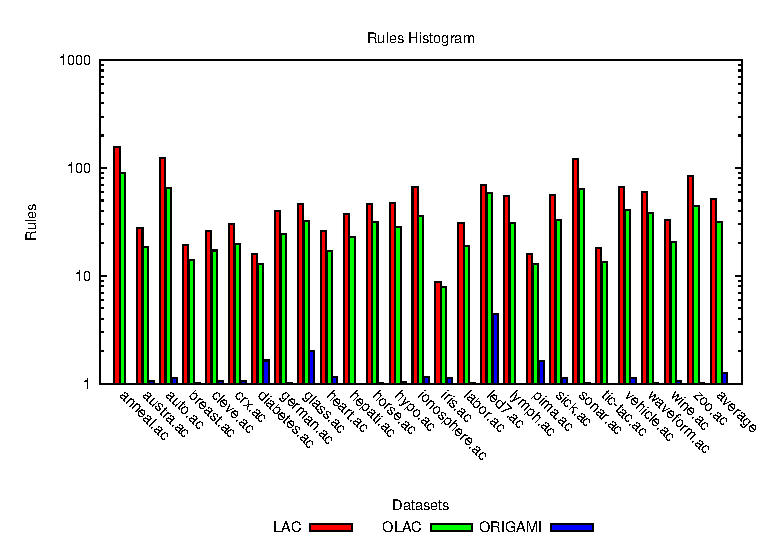
\includegraphics[width=\textwidth]{../thesis/graphs/histogram_best_run_for_avg_db_rul_en}
	\end{centering}
\end{frame}

\begin{frame}[shrink]{Execution Parameters}
	\begin{centering}
	\begin{table}[htbp]
	\centering
		\renewcommand{\tabcolsep}{1.8mm}
		\begin{tabular}{|l|c|c|c|}
		\hline
					& \textbf{LAC}	& \textbf{OLAC}	& \textbf{ORIGAMI}	\\
		\hline
		support			& 0.001	& 0.0001	& 0.0001		\\
		\hline
		confidence		& 0.01		& 0.0001	& 0.0001		\\
		\hline
		min-num-rules		& 1		& 1		& 1			\\
		\hline
		max-num-rank-rules	& 1000		& 100		& 10			\\
		\hline
		min-rule-len		& 1		& 1		& -			\\
		\hline
		max-rule-len		& 1		& 2		& -			\\
		\hline
		rule-measure		& n		& n		& c			\\
		\hline
		orth-metric		& -		& s		& s			\\
		\hline
		orth-method		& -		& s		& -			\\
		\hline
		orth-pat-ordering	& -		& s		& -			\\
		\hline
		origami-alpha		& -		& -		& 0.1			\\
		\hline
		origami-beta		& -		& -		& 0.8			\\
		\hline
		\end{tabular}
	\caption{Best Parameters for Each Run}
	\label{tab:best_parms_for_avg_db}
\end{table}
	\end{centering}
\end{frame}

\begin{frame}
	\begin{block}{Results obtained with LAC using the best parameters for OLAC}
		Patterns: $249.03$ \\
		Rules: $628.12$ \\
		Accuracy: $0.54$
	\end{block}
\end{frame}

\begin{frame}[shrink]{Comparing the Results}
	\begin{centering}
	\begin{table}[htbp]
	\centering
%		\resizebox{0.95\textwidth}{!} {
		\begin{tabular}{|l|c|c|c|c|}
		\hline
				& \textbf{OLAC}		& \textbf{OLAC}			& \textbf{$\neg$ OLAC}	& \textbf{$\neg$ OLAC}	\\
		\textbf{Datasets}	& \textbf{\&}		& \textbf{\&}			& \textbf{\&}			& \textbf{\&}			\\
				& \textbf{LAC}		& \textbf{$\neg$ LAC}		& \textbf{LAC}			& \textbf{$\neg$ LAC}		\\
		\hline
		anneal.ac       & 95.11         & 1.13               & 0.75                     & 3.01                          \\
		\hline
		austra.ac       & 84.93         & 1.88               & 1.45                     & 11.74                         \\
		\hline
		auto.ac         & 39.51         & 6.83               & 4.39                     & 49.27                         \\
		\hline
		breast.ac       & 96.28         & 0.29               & 1.00                     & 2.43                          \\
		\hline
		cleve.ac        & 81.19         & 1.32               & 1.98                     & 15.51                         \\
		\hline
		crx.ac          & 84.93         & 1.59               & 1.88                     & 11.59                         \\
		\hline
%		diabetes.ac     & 76.82         & 1.04               & 1.30                     & 20.83                         \\
%		\hline
%		german.ac       & 70.40         & 3.40               & 3.10                     & 23.10                         \\
%		\hline
%		glass.ac        & 63.08         & 4.21               & 1.40                     & 31.31                         \\
%		\hline
%		heart.ac        & 82.96         & 0.37               & 1.48                     & 15.19                         \\
%		\hline
%		hepati.ac       & 85.16         & 1.94               & 0.00                     & 12.90                         \\
%		\hline
%		horse.ac        & 70.38         & 3.53               & 3.26                     & 22.83                         \\
%		\hline
%		hypo.ac         & 97.94         & 0.06               & 0.09                     & 1.90                          \\
%		\hline
%		ionosphere.ac   & 90.03         & 1.14               & 2.56                     & 6.27                          \\
%		\hline
%		iris.ac         & 94.00         & 0.67               & 0.67                     & 4.67                          \\
%		\hline
%		labor.ac        & 89.47         & 1.75               & 3.51                     & 5.26                          \\
%		\hline
%		led7.ac         & 61.72         & 4.31               & 4.97                     & 29.00                         \\
%		\hline
%		lymph.ac        & 79.73         & 2.70               & 0.68                     & 16.89                         \\
%		\hline
%		pima.ac         & 76.82         & 0.52               & 1.04                     & 21.61                         \\
%		\hline
%		sick.ac         & 97.04         & 0.04               & 0.18                     & 2.75                          \\
%		\hline
%		sonar.ac        & 80.29         & 2.40               & 2.88                     & 14.42                         \\
%		\hline
%		tic-tac.ac      & 56.47         & 6.78               & 3.86                     & 32.88                         \\
%		\hline
%		vehicle.ac      & 56.86         & 6.50               & 2.72                     & 33.92                         \\
%		\hline
%		waveform.ac     & 71.12         & 6.74               & 1.54                     & 20.60                         \\
%		\hline
		$\vdots$        & $\vdots$      & $\vdots$           & $\vdots$                 & $\vdots$                      \\
		\hline
		wine.ac         & 96.07         & 0.00               & 2.81                     & 1.12                          \\
		\hline
		zoo.ac          & 73.27         & 0.99               & 0.00                     & 25.74                         \\
		\hline
		average         & 78.91         & 2.39               & 1.90                     & 16.80                         \\
		\hline
		\end{tabular}
%		}
	\caption{Comparison between LAC and OLAC (number of correct and wrong classifications)}
	\label{tab:comparison_lac_olac}
\end{table}

	\end{centering}
\end{frame}

% O Aplicativo olac
% Exemplo de Execu��o
% Experimentos

\section{Conclusions}
\subsection{Results}

\begin{frame}{Accuracy}
	\begin{itemize}[<+-| alert@+>]
		\item With orthogonality based approaches we got good results, very close to the classical approach one:
		\begin{itemize}[<+-| alert@+>]
			\item Considering the best parameters for each dataset, the values for accuracies obtained by LAC, OLAC and ORIGAMI were, respectively, $0.843$, $0.840$ e $ 0.839$;
			\item Considering the best parameters for the average of the results, the values for accuracy obtained by LAC, OLAC and ORIGAMI were, respectively, $0.808$, $0.813$ e $0.782$.
		\end{itemize}
	\end{itemize}
\end{frame}

\begin{frame}{Patterns}
	\begin{itemize}[<+-| alert@+>]
		\item The number of patterns used to generate the rules by the orthogonal approaches were lower than by the classical approach:
		\begin{itemize}[<+-| alert@+>]
			\item Considering the best parameters for each dataset, the number of patters used by LAC, OLAC and ORIGAMI were, respectively, $213$, $12$ e $12$;
			\item Considering the best parameters for the average of the results, the number of patterns used by LAC, OLAC and ORIGAMI were, respectively, $19$, $12$ e $1$.
		\end{itemize}
	\end{itemize}
\end{frame}

\begin{frame}{Rules}
	\begin{itemize}[<+-| alert@+>]
		\item The number of rules generated by the orthogonal approaches were much lower than by the classical approach:
		\begin{itemize}[<+-| alert@+>]
			\item Considering the best parameters for each dataset, the number of rules generated by LAC, OLAC and ORIGAMI were, respectively, $628$, $25$ e $23$;
			\item Considering the best parameters for the average of the results, the number of rules generated by LAC, OLAC and ORIGAMI were, respectively, $51$, $31$ e $1$.
		\end{itemize}
	\end{itemize}
\end{frame}

\begin{frame}{Other Results}
	\begin{itemize}[<+-| alert@+>]
		\item The orthogonality metric based in pattern structure obtained the best results;
		\item The association rule metrics that obtained the best results were conviction by LAC and OLAC and confidence by ORIGAMI;
		\item Most of fails found in classification based in orthogonality was not caused by the low orthogonality metric. They were found because sometimes, the different patterns used, induced the results to the wrong class.
	\end{itemize}
\end{frame}

\subsection{Future Works}

\begin{frame}{Next Steps}
	\begin{itemize}[<+-| alert@+>]
		\item Use orthogonality in another points of a classification algorithm;
		\item Research for new heuristics of orthogonal patterns extraction, in order to improve performance;
		\item Research for new algorithms of frequent pattern mining that consider  orthogonality while generating the frequent patterns;
		\item Use of a hybrid approach OLAC-ORIGAMI.
	\end{itemize}
\end{frame}

\subsection{End}
\begin{frame}[c]
\begin{center}
\Large
\alert {Questions?}
\Large
\end{center}
\end{frame}


\end{document}
